\section{Decidim}
\label{sec:decidim}

A plataforma Brasil Participativo foi desenvolvida com o \textit{framework Ruby on Rails} utilizando a \textit{gem Decidim}. Segundo a própria documentação disponibilizada pela comunidade de contribuidores do \textit{Decidim}, a \textit{gem} é descrita como um \textit{framework} que visa possibilitar que qualquer pessoa possa criar uma plataforma \textit{web} para ser utilizada como rede política para participação democrática. O \textit{Decidim} fornece a organizações a capacidade de criar processos para planeamento estratégico, orçamento participativo, concepção colaborativa de regulamentos, espaços urbanos e processos eleitorais \cite{decidim-about}.

\subsection{Arquitetura do Decidim}

O \textit{Decidim} possui várias entidades em sua arquitetura. As mais importantes para entendimento de seu funcionamento são os espaços participativos e os componentes, referidos na documentação como \textit{participatory spaces} e \textit{components}, respectivamente. Uma visão macro das entidades do \textit{Decidim} pode ser visto na Figura \ref{fig:arquitetura-decidim}. O \textit{Decidim} armazena dados de cada uma dessas estruturas utilizando a abordagem padrão de aplicações \textit{Rails like}, isto é, utilizando o \textit{Active Record} e persistindo os dados em um banco de dados relacional, o \textit{PostgreSQL}.

\begin{figure}[htbp]
  \centering
  \caption{Arquitetura do \textit{Decidim}}
  \label{fig:arquitetura-decidim}
  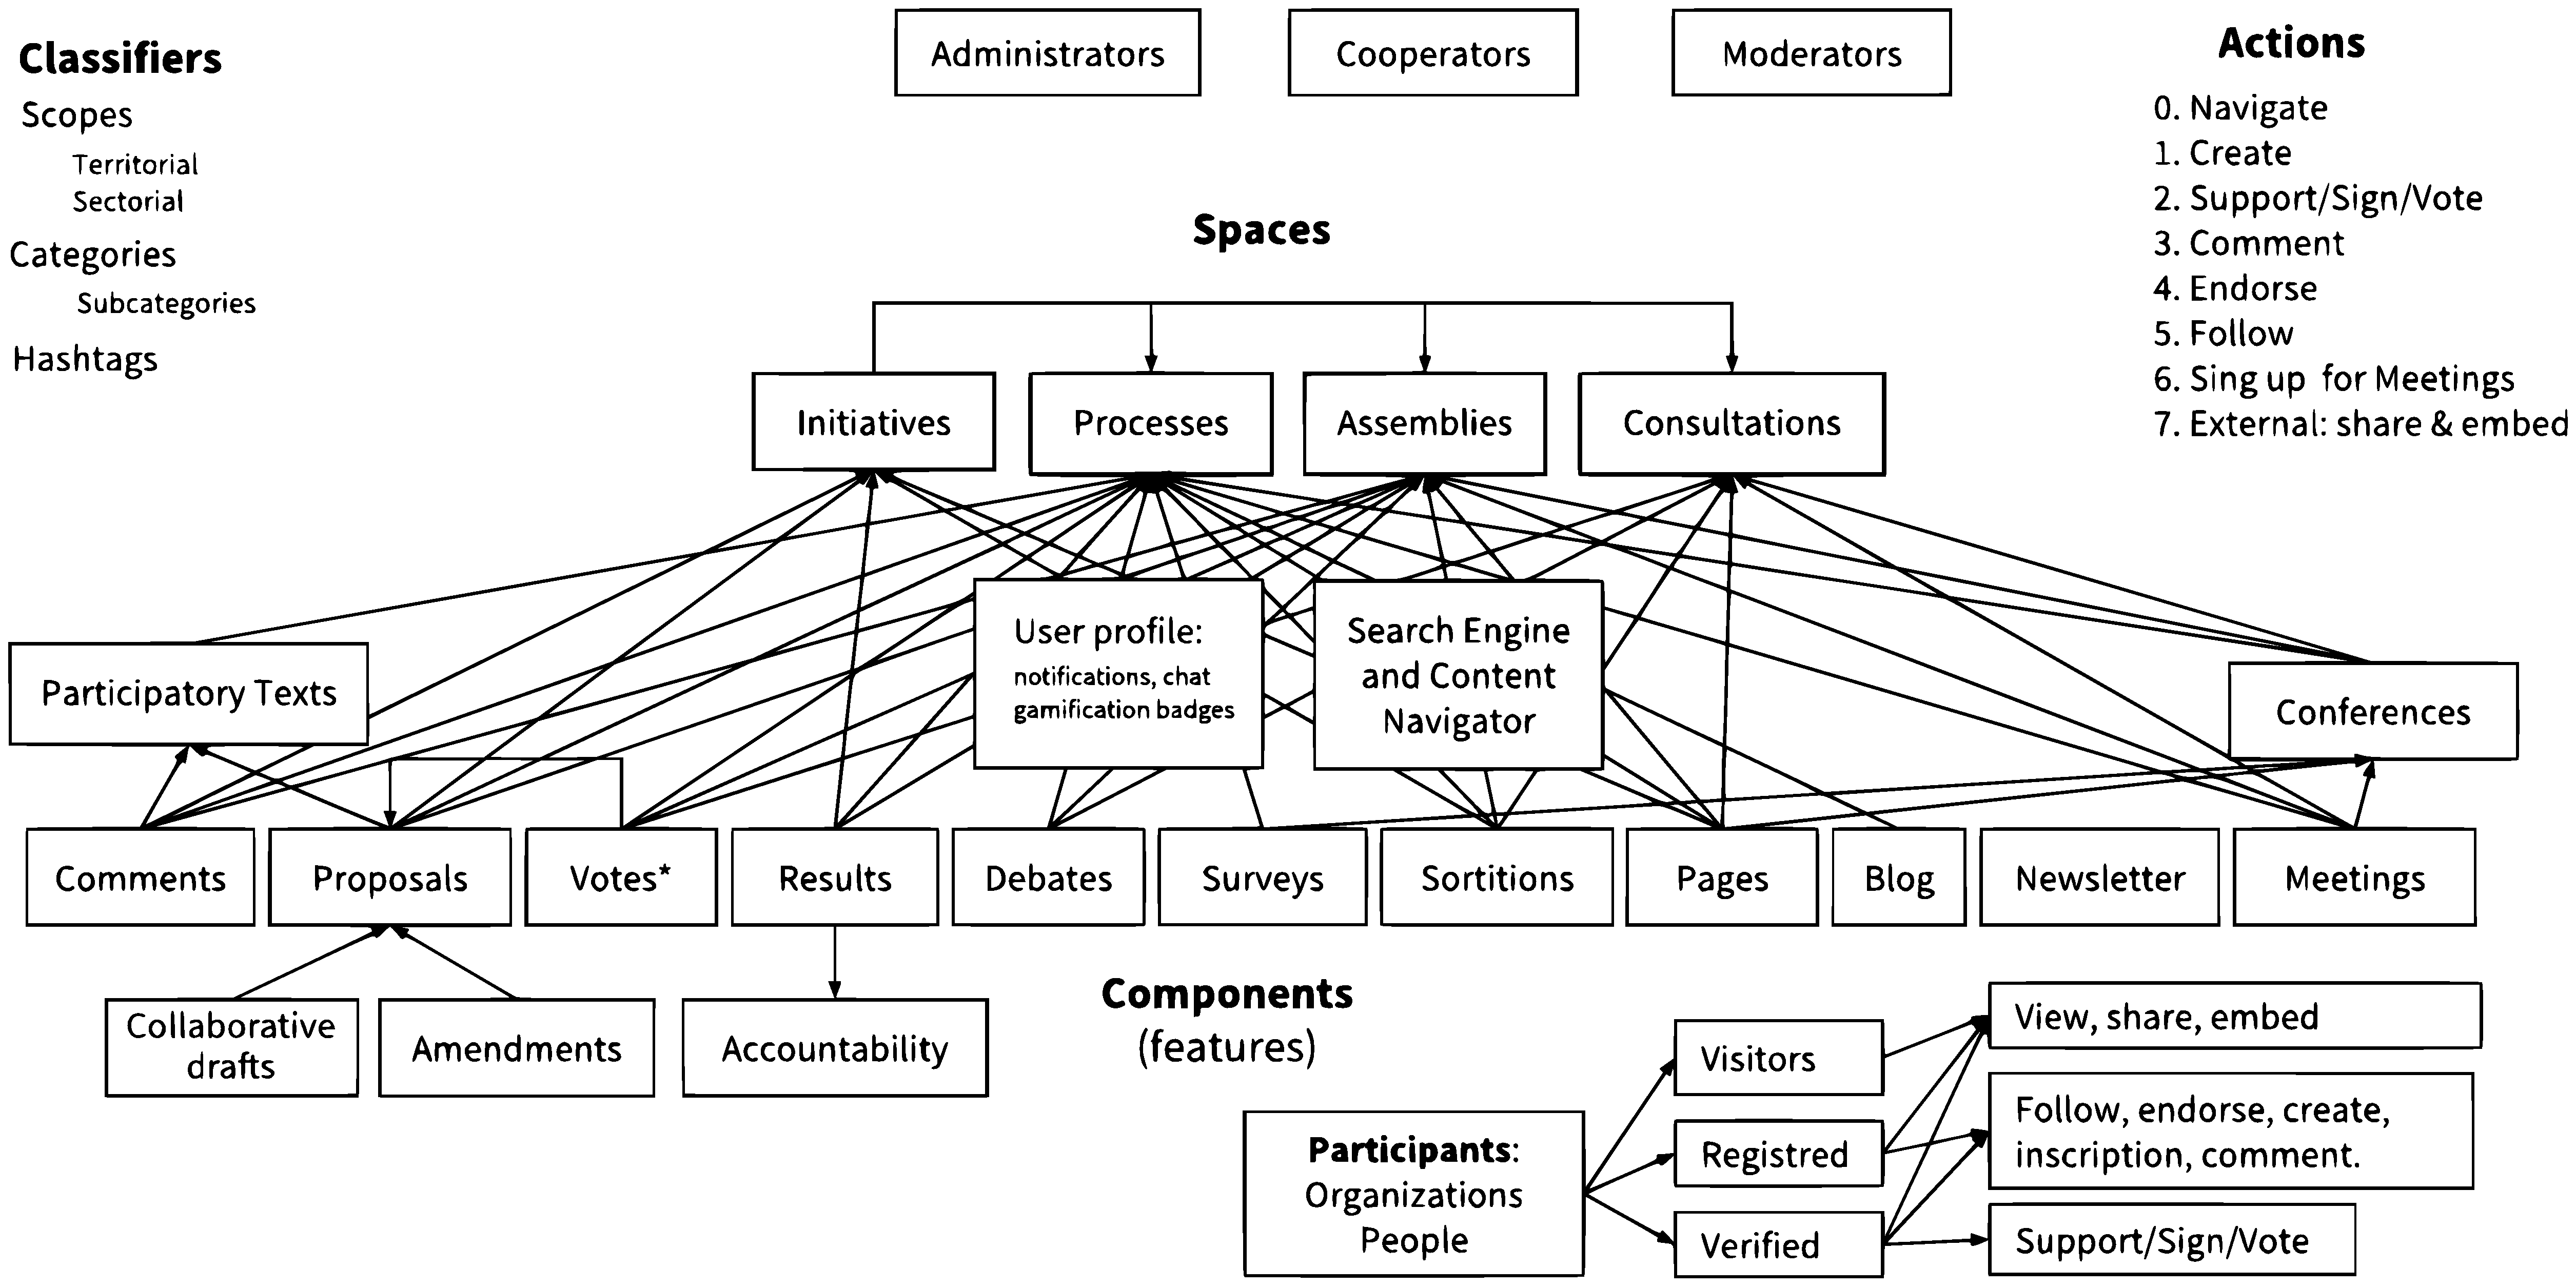
\includegraphics[width=\textwidth]{figuras/diagrama_decidim-min.eps}
  \fonte{\cite{decidim-descriptionpage}}
\end{figure}

\subsubsection{Participatory Spaces}

Os \textit{participatory spaces} são \textit{frameworks} que definem como a participação será realizada, os canais ou meios pelos quais cidadãos ou membros de uma organização podem processar solicitações ou coordenar propostas e tomar decisões. Iniciativas, processos, assembleias e consultas são todos espaços participativos, estes referidos na documentação como \textit{initiatives}, \textit{participatory processes}, \textit{assemblies} e \textit{consultations}, respectivamente. Exemplos específicos incluem: uma iniciativa cidadã para alterar diretamente uma regulamentação; uma assembleia geral ou conselho de trabalhadores; um orçamento participativo, planejamento estratégico ou processo eleitoral; um referendo ou uma convocação para votar "Sim" ou "Não" para mudar o nome de uma organização \cite{decidim-descriptionpage}.

A nível de código, cada implementação de um novo \textit{participatory space} é feita em um submódulo separado em uma \textit{gem} própria. Uma relação entre cada um dos espaços participativos já existentes por padrão no \textit{Decidim} e o seu respectivo submódulo pode ser vista na Tabela \ref{tab:modulos-participatoryspaces}.

\begin{table}
  \centering
  \caption{Módulos dos espaços participativos padrões do \textit{Decidim}}
  \label{tab:modulos-participatoryspaces}
  \begin{tabular}{cc}
    \toprule
    Espaço Participativo & Módulo \\
    \midrule
    Assembleias & decidim-assemblies \\
    Consultas ou Eleição & decidim-elections \\
    Iniciativas & decidim-initiatives \\
    Processos Participativos & decidim-participatory\_processes \\
    \bottomrule
  \end{tabular}
  \fonte{\cite{decidim-descriptionpage}}
\end{table}

\subsubsection{Components}

Os \textit{components} são os mecanismos participativos que permitem uma série de operações e interações entre os usuários da plataforma dentro de cada um dos espaços participativos. No \textit{Decidim} há disponível por exemplo os seguintes componentes: comentários, propostas, debates, pesquisas, sorteios, blogs e reuniões. Outros componentes que se baseiam nos componentes básicos são: textos participativos, responsabilidade e conferências \cite{decidim-descriptionpage}.

Da mesma forma que ocorre com os espaços participativos, os componentes são implementados através de submódulos em formato de novas \textit{gems}. Na Tabela \ref{tab:modulos-components} é possível conferir o nome do módulo de cada componente fornecido por padrão pelo \textit{Decidim}.

\begin{table}
  \centering
  \caption{Módulos dos componentes padrões do \textit{Decidim}}
  \label{tab:modulos-components}
  \begin{tabular}{cc}
    \toprule
    Componente & Módulo \\
    \midrule
    Comentários & decidim-comments \\
    Propostas & decidim-proposals \\
    Debates & decidim-debates \\
    Pesquisas & decidim-surveys \\
    Sorteios & decidim-sortitions \\
    \textit{Blogs} & decidim-blogs \\
    Reuniões & decidim-meetings \\
    \bottomrule
  \end{tabular}
  \fonte{\cite{decidim-descriptionpage}}
\end{table}

\subsubsection {Participatory Texts}

Os \textit{Participatory Texts}, em português: textos participativos, é uma funcionalidade do componente \textit{proposals} que permite o uso de propostas como parágrafos de texto. O seu uso pode ser variado, mas em geral é utilizado para discutir de forma participativa: normativas, planos e outros tipos de texto \cite{decidim-participatory-texts}.